%!TEX root = ../thesis.tex
%*******************************************************************************
%*********************************** Fifth Chapter *****************************
%*******************************************************************************

\chapter{Experimental Procedure}  %Title of the Fifth Chapter
\label{chapter procedure}

\ifpdf
    \graphicspath{{Chapter5/Figs/Raster/}{Chapter5/Figs/PDF/}{Chapter5/Figs/}}
\else
    \graphicspath{{Chapter5/Figs/Vector/}{Chapter5/Figs/}}
\fi

This chapter describes the protocol of the experimental procedure as well as the calculations performed to quantify the measurements obtained during the test. City University London Research Ethics Committee approved the experimental procedure and protocol. Examination authorised under reference \textit{''SREC 15-16 01 E 29 09 201''} of the \nth{11} of November 2015. 

In this study, nine healthy volunteers participated where six were males and three females aged between \numrange{23}{37} years-old (mean 28.77). As per regulation of the committee, only healthy participants took part of the research. Any participant with cardiovascular disease history did not take in the study. 

Previous to the recruitment of participants, they received documentation explaining the whole procedure. Once they agreed, the party returned the consent form signed to schedule the study. The experiments took place at the Research Centre for Biomedical Engineering of City, University of London. Upon arrival partaker acclimatised for \SI{10}{\min} which room temperature was \SI{22(2)}{\degreeCelsius}. During this period, it was clearly explained the experimental procedure to the attendant. Then the following steps took place.


%********************************** %First Section  **************************************
\section{Experimental procedure} %Section - 5.1
\label{section procedure 1}

After filling paperwork and completing acclimatisation different instruments were used to acquired physiological signals. These measurements included ECG, PPG, laser Doppler flowmeter, Doppler ultrasound and impedance plethysmography. Table \ref{table:instruments} describes the purpose of each instrument in this experiment. 

\begin{table}
	\caption{Instruments used during the study and function}
	\centering
	\label{table:instruments}
	\begin{tabu}{ccp{4.5cm}}
		\hline 
		\textbf{Instrument} & \textbf{Method} & \textbf{Measurement} \\\tabucline[2pt]{-}
		ECG & Sense of electrical charges in heart & Electrocardiogram \\\hline 
		PPG & Optical & Measurement of changes of volume in vascular bed \\\hline 
		LDF & Optical & Measurement flow in capillary bed (Cell level) \\\hline 
		iPG & Electrical & Measurement of changes of volume in a segment \\\hline
		Doppler Ultrasound & Electromagnetic & Measurement of flow speed \\\hline 
	\end{tabu}  
\end{table}

The ECG device used for taking the electrocadiographic was a Cardioline\textsuperscript{\textregistered} Delta 60 plus \cite{remco:delta60} using a 4 electrodes configuration. The PPG device registering the photo-plethysmography waveform was the Zen PPG, using a finger sensor operating with a light source at \SI{680}{\nano\meter}.  The LDF instrument used in this experiment was the moor VMS-LDF2 \cite{moor:LDF2}. This instrument operates with a laser light at a wavelength of \SI{785}{\nano\meter}. The Doppler ultrasound utilised was a Huntleigh Healthcare MD2 instrument with a sensor head of \SI{8}{\mega\hertz} \cite{ht:MD2}. Finally, the iPG device described in the previous section was used to take the impedimetric readings. 

%**********************************% Subsection 5.1.1  *************************************
\subsection{Instruments set-up}
\label{section procedure 1.1}

Before attaching any instruments to the participants, it is required to take physical dimensions from them. This data is needed to convert into meaningful numbers some of the physiological measurements. For instance, the quantification of impedance plethysmography requires to know the geometric shape of the volume being measured. Hence, it is needed recording the forearm's segment volume by weighing length and circumference. Additionally, the distance from the heart to shoulder, upper arm length, and shoulder to index finger length was also recorded as reference points. 

Then, all the participants sat in a comfortable chair. Their left arm rested on a soft cushion on a table next to a chair adjusted to collaborator's height. After that, blood pressure was taken using an automated instrument, recording diastolic and systolic values for each one. Next, each participant placed four ECG electrodes on themselves, forming an Einthoven triangle. According to the device's instructions, electrodes must be placed one on each shoulder and ankle. Then, leads were secured to the electrodes verifying that ECG signal was clean. The apparatus includes an output port that exports the waveform for further processing. 

Following this step, a PPG probe was placed on the index finger. The PPG instrument used is a device designed by the biomedical research group of City University known as Zen PPG. This equipment has two channels available, but the experiment only required one port. Each channel provides two outputs containing AC and DC components of the photoplethysmography waveform. 

%\mynote{Check for the type of probe used. Nellcor?}

In the next step, the laser Doppler Flowmetry probe~\cite{moor:LDF2} was attached on the mid-section of the forearm. This device detects moving red blood cells within a vessel under the vascular bed in the skin. This device also has an external analogue port where the signal acquired can be exported for post-processing.  

Next, the Ultrasound Doppler probe was placed as close as possible to the radial artery. When the probe is placed closed to a main vessel the speed of blood flow produces a unique audible signal. However, calculating blood flow form this signal requires a set of skills by placing the probe at a fix angle and closeness to the artery to be measured. Therefore, the probe head of the instrument needs to be placed at a fixed angle. Hence, the instrument's head was secured using a laboratory stand and clamp pointing at the party's radial artery on the wrist. The appliance also provides an external port for additional processing.  

Finally, the impedance plethysmography electrodes were placed on the forearm's skin. For this, ECG electrodes were utilised as they a provided good contact essential for the experiment to be carried out successfully. The current probes were placed following the path of the left radial artery, one below the elbow (brachial artery) and a second on top of the radial artery close to the wrist. The potential electrodes were located next to the previous electrodes towards the internal side of the forearm. The diameter of the circumference around these electrodes as well as its distance separation was recorded. With this physical measurements is possible to calculate the volume of the forearm's segment to be measured. The total volume of that portion of the arm was calculated using equation \ref{eq:v_e}.

\begin{align}
	\label{eq:v_e}
	V_e =\frac{l \times (C_1^2+C_1 \times C_2 + C_2^2)}{(12 \times \pi)} \tagaddtext{[\si{\cubic\centi\meter}]}
\end{align}

where $V_e$ is segment's volume, $l$ is the length between the potential electrodes, $C_1$ and $C_2$ are the circumference measurement at elbow and wrist electrodes respectively.

The whole experiment set-up can be seen on figure \ref{fig:experimental set-up} where all the instruments and its positions are noted.

\begin{figure}[!htpb]
	\centering
	\includegraphics[width=15cm,keepaspectratio]{figure1}
	\caption{Position of instruments during the experiment}
	\label{fig:experimental set-up}
\end{figure}

%%********************************** % Section 5.1.2 ******************************************
\subsection{Physiological measurements}
\label{section procedure 1.2}
As noted before, at the beginning of the study physiological measurements were taken from the participants. Data such age, sex and arm to hearth distance were collected initially. The table \ref{tbl:physiological} summarise the information provided by each of the participants. In total, three female and six male participants took part of the study. Their ages ranged between \SIrange{23}{37}{year-old} (mean \num{29.12(494)}). 

\begin{table}[!ht] %tbl:physiologica
	\caption{Participants' forearm measurements and initial volume.}
	\label{tbl:physiological}
	\centering
	\begin{tabular}{lcc|ccc}
		\toprule
		&              &              &         \multicolumn{3}{c}{\textbf{Dimensions [\si{\cm}]}}         \\
		& \textbf{Age} & \textbf{Sex} & \textbf{Arm length} & \textbf{Shoulder} & \textbf{Total length} \\
		&              &              &                     &  \textbf{to heart}   &                       \\ \midrule
		Participant 1 &      26      &     Male     &         80          &          26          &          106          \\
		Participant 2 &      23      &    Female    &         66          &          24          &          90           \\
		Participant 3 &      27      &    Female    &         74          &          24          &          98           \\
		Participant 4 &      37      &     Male     &         68          &          24          &          92           \\
		Participant 5 &      29      &    Female    &         62          &          24          &          86           \\
		Participant 6 &      36      &     Male     &         70          &          24          &          94           \\
		Participant 7 &      29      &     Male     &         73          &          23          &          96           \\
		Participant 8 &      26      &     Male     &         69          &          23          &          92           \\ \bottomrule
	\end{tabular}
\end{table}

Additionally to these measurements, the distance between impedance potential electrodes and the arm circumference at the same point was also recorded using a measuring tape. With this data is possible to estimate the forearm's segment total volume by measuring the distance between the potential electrodes ($l$), and the circumference on the location of each electrode (C$_1$ and C$_2$). Table \ref{tbl:measurments} shows the dimensions of the participant's forearm between the sensing electrodes and the segment's volume calculated from Equation \ref{eq:v_e}.

Taking these dimensions with a measuring tape may induce some errors in the data. For instance, applying too much pressure towards the arm when taking the measurement may read a lower circumference value. However, it allows estimating the initial volume of the forearm segment which represents the original volume of the conductive portion. 

\begin{table}[!htbp] %tbl:measurments
	\caption{Participants' forearm measurements and initial volume.}
	\label{tbl:measurments}
	\sisetup{separate-uncertainty=true}
	\centering
	\begin{tabular}{lcccccc    S[table-format=2.2]@{\,\( \pm \)\,}S[table-format=1.2]}
		\toprule
		&  \textbf{L [\si{\cm}]}   &  \textbf{C$_1$ [\si{\cm}]}  &  \textbf{C$_2$ [\si{\cm}]}  &   \textbf{Ve [\si{\cubic\cm}]} \\\midrule
		Participant 1 & 14.8 & 17.5 & 27.5 & 606.05 \\
		Participant 2 & 11.0 & 15.0 & 20.0 & 269.90 \\
		Participant 3 & 13.0 & 19.0 & 26.5 & 540.27 \\
		Participant 4 & 10.0 & 17.5 & 25.0 & 363.07 \\
		Participant 5 & 10.0 & 17.5 & 23.5 & 336.81 \\
		Participant 6 & 11.0 & 18.5 & 27.0 & 458.32 \\
		Participant 7 & 13.5 & 15.0 & 23.0 & 393.55 \\
		Participant 8 & 11.5 & 17.0 & 23.5 & 378.49 \\ \bottomrule
	\end{tabular}
\end{table}

%********************************** %Third subection *************************************
\subsection{Experimental protocol}
\label{section procedure 1.3}

One of the aims of this experiment is to look into iPG waveform's alterations when there is an obstruction in the blood flow in the forearm. It is possible to restrict the blood circulation to this area by applying a mechanical blockage in the upper arm using an standard inflatable blood pressure instrument. The device used necessitates being pumped manually using an inflation bulb. A gauge in the instrument indicating the cuff's pressure level. The cuff was secured to the left biceps of the participant. 

The protocol required recording three different types of blood flow occlusion. The first kind restricts the blood flow return by blocking the venous circulation. This method is widely used to assess peripheral circulatory problems as described by Wilkinson et al. \cite{wilkinson2001venous}. This obstruction can be produced by inflating the cuff usually just below diastolic pressure between \SIrange{10}{20}{\mmHg}. Thus, blocking the upper arm obstructs the blood flowing within the median cubital and basilic veins without obstructing the arterial inflow of the brachial artery.  Overall, for each participant, the target pressure was \SI{20}{\mmHg} under their diastolic pressure recorded at the beginning of the session.

The second class of blood flow limitation was a partial arterial occlusion. This kind of blockage decreases the amount of arterial blood coming into the forearm but also stops venous blood return, studies have demonstrated that constricting an artery reduces the arterial flow towards the periphery \cite{uchida1977cyclical}. As an illustration, this can be obtained by applying a mechanical compression to the upper arm between diastolic and systolic pressures, increasing the wall pressure of the brachial artery. Therefore, the objective was to constrict the upper arm about the mean value between diastolic and systolic pressure. For that, it was calculated using the following equation.

\begin{align}
	\label{eq:meanpressure}
	P_m = \frac{P_d + P_s}{2} \tagaddtext{[\si{\mmHg}]}
\end{align}

where $P_d$ is diastolic pressure and $P_s$ is systolic pressure. 

The last kind of occlusion needed is total occlusion, which is possible to obtain by occluding above systolic pressure. Also known as  “Suprasystolic” or “stop-flow” can provides valuable tonometric information \cite{lowe2009non}. In this experiment, blood flow was blocked by inflating the cuff above \SI{20}{\mmHg} of participant's systolic value previously measured. This method of occlusion completely restricts the inflow and outflow of venous and arterial blood. Hence, it is expected that no change of volume takes place all along this part of the test.

\subsubsection{Blood pressure occlusion estimation}
Finding these blood pressure levels requires to measure and record the blood pressure for each participant. Therefore, before starting the study, three readings of blood pressure were taken and averaged per participant using an automated blood pressure instrument brand Omron IntelliSense (Omron Healthcare). The mean systolic and diastolic pressures of all the partakers of the investigation were \SI{116.25(1366)}{\mmHg} and \SI{72.75(723)}{\mmHg} respectively. The venous occlusion level was targeted to \SI{20}{\mmHg} below systolic pressure the total mean was \SI{55.00(801)}{\mmHg}, the partial arterial pressure was calculated using equation \ref{eq:meanpressure}, the average was about \SI{94.63(1021)}{\mmHg} and total occlusion was around \SI{136.25(1367)}{\mmHg}. Table \ref{tbl:occlusions} details the blood pressures recorded per participant.

\begin{table}[!htbp] %tbl:occlusions
	\caption[Blood pressure and occlusion levels of the participants]{Participants' initial blood pressure and levels for venous, partial arterial and total occlusion.}
	\label{tbl:occlusions}
	\centering
	\begin{tabular}    {lcccc}
		\toprule
		& \textbf{Blood pressure}  &  \textbf{Occlusion 1}   & \textbf{Occlusion 2}  &  \textbf{Occlusion 3} \\
		&  [\si{\mmHg}]   &        [\si{\mmHg}]  &    [\si{\mmHg}]   &  [\si{\mmHg}]\\ \midrule
		Participant 1  &  124/78   &        50  &    101   &  144\\ 
		Participant 2  &  105/65   &        50  &     85   &  125 \\
		Participant 3  &  120/78   &        60  &     99   &  140 \\
		Participant 4  &  120/72   &        60  &     96   &  140 \\
		Participant 5  &  100/60   &        40  &     80   &  120 \\
		Participant 6  &  143/82   &        60  &    113   &  163 \\
		Participant 7  &  107/73   &        65  &     90   &  127 \\
		Participant 8  &  111/74   &        55  &     93   &  131 \\\bottomrule
	\end{tabular}
\end{table}

With the data from table \ref{tbl:occlusions} was possible to set the parameters for the experimental procedure. The column \textit{occlusion 1} establishes the proper pressure for venous occlusion plethysmography (VOP). With the pressures from column \textit{occlusion 2} the arterial blood flow was restricted as well as the venous return. Finally, \textit{occlusion 3} provides information of changes of impedance during total occlusion.

%********************************** %Second subection *************************************
\subsection{Data acquisition}
\label{section procedure 1.4}

All the instruments used in the experiment provided external ports for further data processing. These output ports were connected to a DAQ NI-6211 (National Instruments). This analogue to digital converter card provides 32 channels and a combined sampling rate of \SI{250}{\kilo\sample\per\second}. The DAQ connects to a personal computer via USB port (Version 1.0). All the signals were sampled at \SI{1}{\kilo\hertz} with a reference voltage between \SIrange{0}{10}{\volt} for the iPG channel $Z_{DC}$ and \SI{\pm 5}{\volt} for the other signals. Therefore, the resolution of the DAQ was \SI{152.6}{\micro\volt}, which it was calculated using equation \ref{eq:resolution}. 

\begin{align}
	\label{eq:resolution}
	Res =\frac{V_{p-p}}{2^{n}}		\tagaddtext{[\si{\volt}]}
\end{align}

where $V_{p-p}$ is the reference voltage peak to peak and $n$ is the number of bits used to sample the signal. 

A virtual instrument using LabView \cite{LabView:2016} was created for displaying, processing and storing raw data. Figure \ref{fig:experimental set-up 2} shows the front-end of the program. The programmed custom virtual instrument shows four channels of waveforms. For the purpose of the experiment iPG, ECG, PPG and Ultrasound Doppler were those selected for portraying the signals.

\begin{figure}[!htpb]
	\centering
	\includegraphics[width=15cm,keepaspectratio]{figure2}
	\caption{Additional instruments used during the experiment}
	\label{fig:experimental set-up 2}
\end{figure}

For displaying purposes, a band-pass filters were applied to the iPG and PPG signals removing unwanted DC components and high frequency noises. The waveforms from the other instruments did not require filtering as the devices provided a clean signal. 

The virtual instrument also included configuration capabilities. Two tabs within the program provided field for partaker's physical measurements, general application settings and adjustment for the PPG instrument. The participant tab required the following data: left arm dimensions, blood pressure and file path name. In the second tab, the VI adjusts the light intensity of the PPG probe. Usually a \SI{20}{\milli\ampere} is enough to provide a good amplitude signal. At the end of the experimental procedure, all raw data was stored on an LVM file created by LabView.

The main panel apart from just displaying waveforms also includes control buttons and a timer.  Pressing the start button commences a timer and stores the data waveform in memory. Pushing on the same button again stops the timer and saves all the data in a local LVM file. 

%\mynote{Add proper description of the DAQ used, including channels}

\subsubsection{Recording waveforms}
At this point, after all the physiological measurements were recorded and the instruments were operating successfully, a small test took place. While waveforms were being shown on screen, \SI{2}{\min} of recordings were taken but not recorded yet. Participants were advised to limit their movements during the experiment. 

As soon as all signals were readable and free of noise, the start button of the VI was pushed to initiate the study. In the beginning, \SI{5}{\min} of baseline recordings were obtained. These waveforms provided the standard control wave to compared with occluded waveforms. Then, immediately after the timer reached this time the cuff was inflated rapidly to \SI{20}{\mmHg} below diastolic pressure. Therefore, producing venous occlusion and an increment in the total volume of the forearm because of the blood pooling effect. This level of blockage was held for \SI{3}{\min} followed by swiftly deflating the cuff. 

The next step of the experiment required to produce the partial arterial occlusion, using similar time spans as the ones during venous occlusion. As described in the literature reperfusion after an occlusion does not affect blood pressure, heart rate or blood flow \cite{kharbanda2002transient}. Hence, \SI{5}{\min} is enough time  to restore the blood flow to normal limits. For this reason, the cuff's air valve was left open bleeding all the air contained inside. After this period, the cuff was quickly inflated again until reaching the pressure calculate in equation \ref{eq:meanpressure}. The cuff's pressure was maintained at this level for \SI{3}{\min} proceeded by a quick pressure release. 

Last, for the purpose of total blood occlusion a similar method, was applied. One more time, \SI{5}{\min} of baseline waveforms were taken followed by a fleeting cuff inflation to \SI{20}{\mmHg} above diastolic pressure. This compression was kept for \SI{3}{\min}. At this point, maintaining this tourniquet effect can be painful after a couple of minutes. As a result, some of the helpers ended up re-accommodating and producing motion artefacts in the data. 

Finally, the last \SI{5}{\min} of baseline waveforms were recorded to study the recovering effect. When time was up, the stop button was pushed on saving all the data onto an LVM file for further processing in Matlab. Figure \ref{fig:pressure applied} shows the pressure levels applied during the whole experiment.

\begin{figure}[!htpb]
	\centering
	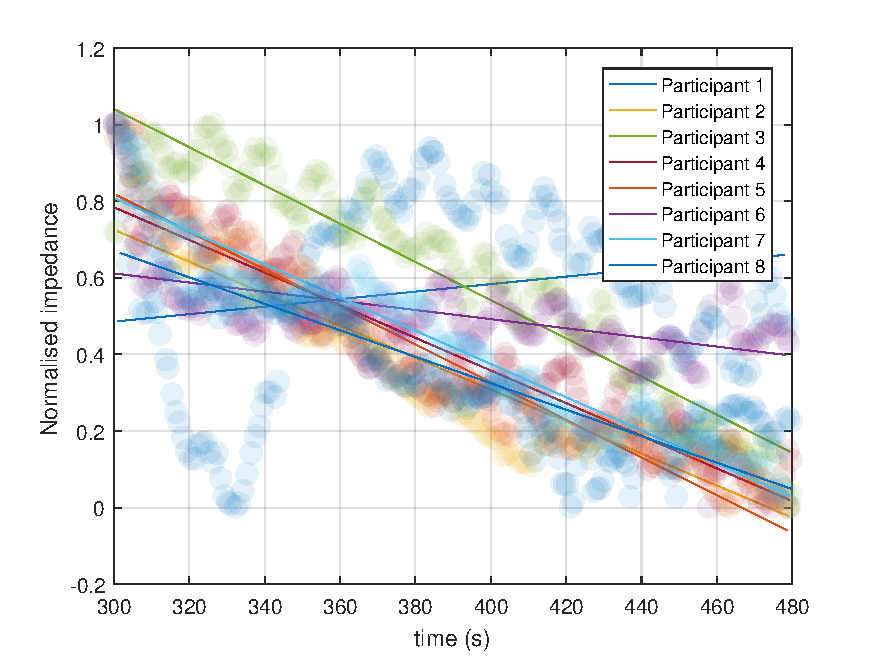
\includegraphics[width=15cm,keepaspectratio]{figure3}
	\caption{Pressure applied to the participant during the experiment. The clear areas represent the resting period of \SI{5}{\minute}, the shaded areas represent the pressure applied at the desired level during \SI{3}{\minute}}
	\label{fig:pressure applied}
\end{figure}

%********************************** % Section section 5.3******************************************
\section{Data processing}
\label{section procedure 2}
Once all the data was collected and saved in the LVM format, the waveforms were post-processed in Matlab \cite{MATLAB:2016}. In more detail, a Graphic User Interface (GUI) Matlab program was created capable of comparing four waveforms at the same time while applying filters, finding peaks and windowing sections of data. A front-end of the application can be seen in figure \ref{fig:Matlalb Interface}.

Importing the LVM file into Matlab requires only to extract the most relevant information. Therefore, a parsing program was created where unwanted headers and columns of unnecessary data were removed. One of the challenges found in the data importing process was the LVM file size. While sampling at \SI{1}{\kilo\hertz} provided great detail of the waveforms, it also created files of approximately \SI{300}{MB}. Importing this file size slowed down the workstation tremendously. For this reason, while importing into Matlab, data was decimated in a magnitude of ten. Consequently, each physiological waveform was reduced to less than \SI{1}{MB} of size while still keeping a good waveform detail. 

This data decimation does not affect the waveform data. In fact, according to Nyquist rate, data was being oversampled. Physiological signals depending on the heart rate are between \SIrange{1}{2}{\hertz}. According to Nyquist theorem up to \SI{4}{\hertz} would have provided enough sampling frequency for the waveforms \cite{nyquist1928certain}. Nevertheless, a sampling of \SI{100}{\hertz} is sufficient to give a high resolution of the discrete-time signal. Even so, having oversampled signals was not a random case. Indeed it allows implementing high order digital filters with sharp cut-off frequencies. 

\begin{figure}[!htpb]
	\centering
	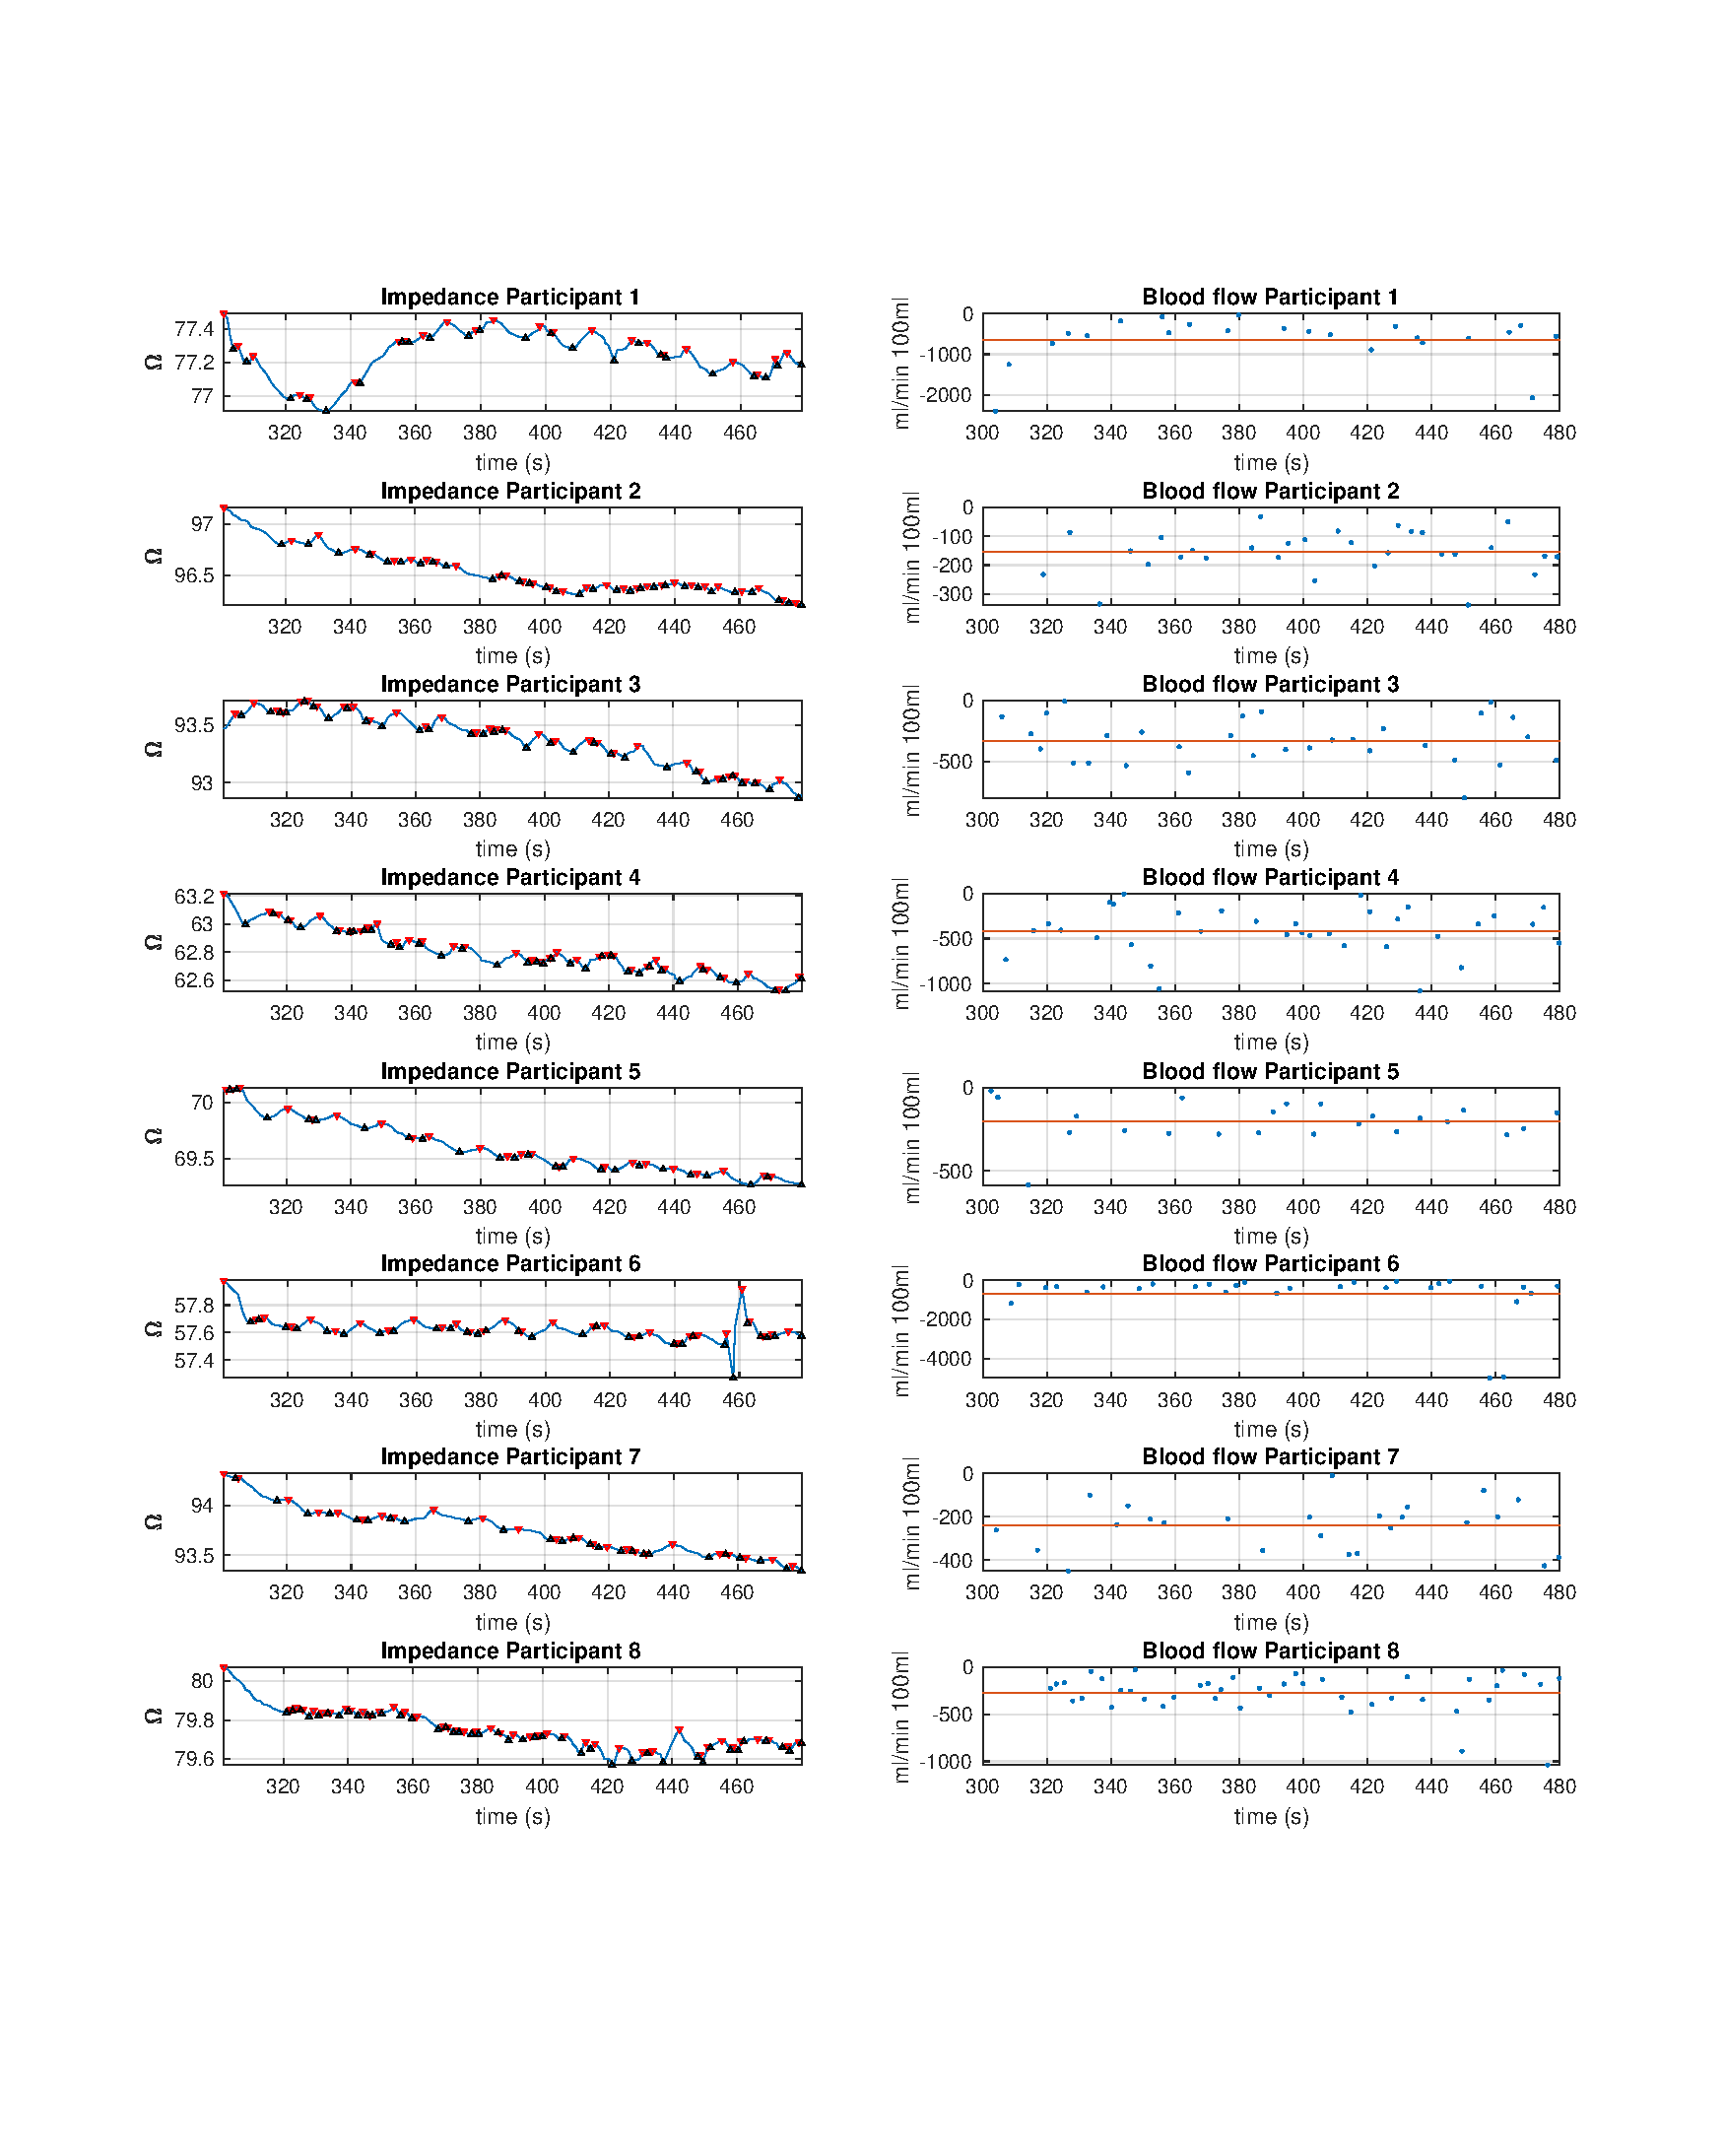
\includegraphics[width=15cm,keepaspectratio]{figure4}
	\caption[Graphic user interface of the Matlab application]{Graphic user interface of the Matlab application used to qualify data and post-processing the signals acquired}
	\label{fig:Matlalb Interface}
\end{figure}

After the decimated data was imported into Matlab, the parsing program converted and saved each waveform into a Matlab file format (.mat). Having the data into this kind of file speeds up the loading in memory of the data as well as the waveform presentation in the GUI. Another advantage of this file conversion is that data processing can be performed online without using extensive computing resources. 

The end data is the representation in volts of the physiological measurements captured during the experiment. For this reason, the information has to be converted into more meaningful data. The following section describes the mathematical process to convert the signals from volts into the equivalent measurements.

%********************************** % Section section 5.2.1******************************************
\subsection{Data conversion}
\label{section procedure 2.1}
The data imported into the GUI is a representation in volts of all the physiological measurements. Therefore, this information must be converted into significant values that represent the physical variable measured. For instance, the signals coming from the port $Z_{DC}$ of the iPG device is only the potential measurement of the forearms, not yet the net impedance. Converting this reading correctly into impedance needs to be divided by the current driven by the device. From this values, another physiological measurements can be derived such as volume and blood flow. On top of this, extra filtering needs to be applied to isolate certain characteristics of the waveforms. 

The same situation applies for the readings from the Ultrasound Doppler and the Doppler Flowmetry. The signals collected are only the raw data in volts which must be converted to the right scale. The following section describes more in detail the mathematical equations and tools used to convert the raw signals effectively.  

\subsubsection{Calculation of the basal impedance value}
Impedance plethysmography signals need to be converted from volts and current values into its standard scale, which is Ohms ($\Omega$). The iPG device has a channel for current sense called $I_{DC}$, which voltage is equivalent to the peak value of the current being delivered by the instrument. The effective electrical current in amperes ($A$) can be calculated by the gain relation of the different stages of the signal path. According to the circuit schematic (see figure \ref{fig:mhc}), the electrical current is being sensed by a \SI{10}{\ohm} resistor $(R_s)$ in the module \textit{Modified Howland Amplifier module} (see section \ref{section MHC}). Then, this signal is amplified by an instrumentation amplifier in the \textit{current and voltage sensing module} (see section \ref{section V&I sense}) which gain $(G_1)$ was fixed to \num{276}. Following the signal path, the waveform is fractioned by the super-diode circuit which acts as a half-wave rectifier in the \textit{envelope detection module} (see section \ref{section envelope}). The hold circuit keeps the DC voltage constant at the output of the signal which is equivalent to the peak value of the current in volts. As a result, the electrical current in amperes can be calculated using the equation \ref{eq:current}.

\begin{align}
	\label{eq:current}
	I = \frac{V_{IDC} \times 2}{R_x \times G_1} = \frac{V_{IDC} \times 2}{276 \times\ 10 \Omega} = \frac{V_{IDC}}{1380 \Omega} \tagaddtext{[\si{\ampere}]}
\end{align}

%\mynote{Add a section in the design of the device showing how current waveform is converted from AC signal to DC and then into a value.}

The second channel of the iPG device labelled $Z_{DC}$ produces a DC voltage tantamount to the impedance of the forearm. Similarly, as the current sense voltage path, this channel also passes through a series of circuits which amplifies the original potential coming from the forearm's segment. Hence, the real voltage detected by the device can be debunked by the different gains involved in the signal path. 

First, the unknown load is sense by the potential electrodes ($E_2$ and $E_3$ in figure \ref{fig:electrode}) which are directly connected to the \textit{voltage sense module} (see section \ref{section V&I sense}). The instrumentation amplifier (AD8421) of this module was configured to a gain \num{35.65}. In the \textit{envelope detection module} (see section \ref{section envelope}), the signal was rectified by the super-diode circuit, halving the signal amplitude. Therefore, the voltage can be deducted by using equation \ref{eq:vzdc}.


\begin{align}
	\label{eq:vzdc}
	V_z = \frac{V_{ZDC} \times 2}{35.65} \tagaddtext{[\si{\volt}]}
\end{align}

where $V_{ZDC}$ is the DC voltage coming from the port $Z_{DC}$.

Finally, the impedance value can be computed by converting the voltage into impedance using Ohm's law \cite{ohm1827galvanische}. This can be achieved by replacing equation \ref{eq:current} and \ref{eq:vzdc} into \ref{eq:impedance}. The GUI programmed in Matlab automatically makes this impedance conversion when the signal is loaded in the GUI. This mathematical operation is done by a point-to-point division between both signals after their gains have been subtracted to their raw values. 

\begin{align}
	\label{eq:impedance}
	Z = \frac{v}{i}=\frac{V_z}{I} \tagaddtext{[\si{\ohm}]}
\end{align}

\subsubsection{Calculation of the Arterial Pulse Amplitude value}
The third channel of the iPG device is the APA signal designated as $Z_{AC}$. This waveform is an amplified version of the dynamic signal contained within $Z_{DC}$. Analysing the signal's path, it is noticeable that two circuits work on the waveform. First of all, it is the circuit from where the signal is originated which is the voltage from port $Z_{DC}$, meaning that the gain described in the previous section also impacts the signal $Z_{AC}$. The second circuit affecting the signal is the band-pass filter in the \textit{envelope detection module} (see section \ref{section envelope}). As it can be appreciated in figure \ref{fig:envelope detector voltage}, this filter has a fixed gain of \num{142.42} and eliminates any DC and high-frequency noise components. Then, the voltage of the plethysmography wave can be found by combining both gains using equation \ref{eq:ViPG}.

\begin{align}
	\label{eq:ViPG}
	V_{APA} = \frac{V_{ZAC} \times 2}{142.42 \times 35.65}=\frac{V_{ZAC}}{2538.66} \tagaddtext{[\si{\volt}]}
\end{align}

where $V_{ZAC}$ is the raw AC voltage coming from the port $Z_{AC}$.

Likewise, the impedance value of the dynamic signal ($Z_{iPG}$) can be calculated using Ohm's law \cite{ohm1827galvanische}, by replacing the APA voltage from equation \ref{eq:ViPG} and the current from equation \ref{eq:current}. In Matlab this impedance value is calculated as soon as the signal is selected by applying this formula.

\begin{align}
	\label{eq:zipg}
	Z_{iPG}=\frac{v}{i} = \frac{V_{APA}}{I} \tagaddtext{[\si{\ohm}]}
\end{align}

\subsubsection{Converting ultrasound to flow}
\label{sectionDU}
The instrument used in this study was a Huntleigh model MD2 with sensor type VP8. The frequency of the transmitter is \SI{8}{\mega\hertz} which is ideal for blood flow estimation. The principle of this device relates to the frequency of a source to its velocity relative to a sensor \cite{surgeonhand2002Hand}. In other words, if an electromagnetic wave is transmitted at a fixed frequency and is reflected by a moving body, then the frequency of the received signal will be shifted \cite{ht:MD2}.  

The device can detect moving blood cells within a vessel. When a cell passes through the electromagnetic beam a frequency shift occurs, which is proportional to the blood flow velocity. Nevertheless, the Doppler shift is also affected by the angle of the head of the probe and the direction of the flow \cite{surgeonhand2002Hand}.

Because the average velocities found in the human body lies within the audible frequency range, the device reproduces this as a sound using an speaker. The apparatus has an output channel that also produce the equivalent analogue signal for further processing. According to the specifications of the instrument a \SI{3.5}{\volt} signal at the output is equivalent to a \SI{8}{\kilo\hertz} shift signal. Using this as a reference, it is possible to calculate the shift frequency using equation \ref{eq:fshift}.

\begin{align}
	\label{eq:fshift}
	f_D = \frac{V_{DU} \times 8 KHz}{3.5V} \tagaddtext{[\si{\hertz}]}
\end{align}  

where $V_{DU}$ is the analogue output voltage of the instrument. 

According to the Doppler equation described in \ref{eq:doppler}, it is possible to find the velocity of a blood cell derived from its frequency shift. However, there is a correction angle $(\theta)$ between the ultrasound beam and the direction of blood flow. For this reason, the head of the sensor was positioned at a \SI{45}{\degree} angle to the radial artery on the wrist.

\begin{align}
	\label{eq:doppler}
	v = \frac{f_D \times C}{2 f_O \times Cos(\theta)} \tagaddtext{[\si{\meter\per\second}]}
\end{align}

where $f_D$ is the Doppler frequency, $C$ is the speed of sound assumed to be \SI{1540}{\meter\per\second}, $f_0$ is the oscillation frequency of the Doppler instrument in this case \SI{8}{\mega\hertz} and $\theta$ the angle between the ultrasound sensor and the target vessel which is \SI{45}{\degree}.\nknote{this paragraph doesnt make sense}

This angle position was locked using a laboratory stand and a clamp. The angle was fixed to \SI{45}{\degree} angle using a goniometer. Nevertheless, this is one of the shortcomings of this method. The angle can be estimated according to the position of the sensor's case but not to the surface of the crystal of the sensor. There is an incident error that cannot be quantified easily. However, for the event of this study, it was assumed that the angle is \SI{45}{\degree}.

Now the blood flow can be computed by converting velocity to flow if the cross section area of the vessel is known, as in equation \ref{eq:flow}. Not knowing this area precisely is another drawback of this method to calculate blood flow accurately. To know the real cross section area of a vessel requires imaging methods such as Doppler Ultrasonography. 

\begin{align}
	\label{eq:flow}
	\dot{Q} = v \times A \tagaddtext{[\si{\cubic\meter\per\second}]}
\end{align}

where $\dot{Q}$ is flow, $v$ is the velocity of the blood cell and $A$ the cross-sectional area of the radial artery.

However, blood flow can be estimated by using the average cross-sectional area of radial arteries in the population. A study has been found that males have slight larger radial arteries diameter than females (\SI{2.3(039)}{\mm} and \SI{2.11(029)}{\mm} respectively)~\cite{ashraf2010size}. These dimensions were used to calculate the blood flow in the present experiment. It is possible to convert this information into a more common scale of litre per minute by multiplying by 60 seconds and converting $m^3$ into litres. 

\begin{align}
\label{eq:flow_l/min}
\dot{Q} = v \times A \times 60 \times 1000 \tagaddtext{[\si{\cubic\meter\per\second}]}
\end{align}

\subsubsection{Converting LDF}
\label{section:ldf}
The Laser Doppler Flowmetry device utilised in the study was the moor VMS-LDF instrument. LDF is a non-invasive optical method to estimate the blood perfusion in the microcirculation. This device uses the same Doppler principle as described in section \ref{sectionDU} but instead of sound, a beam of light is the source. Similarly, when a red blood cell scatters a light of beam, it produces a frequency shift~\cite{fredriksson2007laser}. 

LDF produces a blood perfusion signal that is comparable to the RBC perfusion or also known as flux. The units of this measurement are Blood Perfusion Unit (BPU) which is an arbitrary unit scale. BPU is the product of the mean number of moving blood cells in the small volume under the probe and the average velocity of moving blood cells. 

This instrument provides an output port that allows exporting the waveform. This connector provides a signal between \SIrange{0}{5}{\volt} which varies according to the flux signal. The configuration menu allows modifying the output scale. It provides three steps at a top limit of \SIlist{1000;500;100}{BPU} output for \SI{5}{\volt}. The measurements taken in this study showed being below \SI{100}{BPU}. Hence, using equation \ref{eq:BPU} converts the output voltage into BPU's.

\begin{align}
	\label{eq:BPU}
	BPU = \frac{V_{BPU} \times 100}{5 V}
\end{align}


%********************************** % Swction section 5.3.2******************************************
\subsection{Digital filtering}
\label{section procedure 3.2}

The signals obtained from the devices contained variable sources of noise. These included respiration, mains noise, motion, high-frequency noise from the iPG current source (\SI{30}{\kilo\hertz}). To remove these sources of different noise, filters were designed in Matlab for post-processing. The command \textit{designfilt} can create a variety of different filters. In the GUI, any user can apply any filter on demand to any signal available. Table \ref{table:filters} gives an overview of the filters that were designed and made available for processing the waveforms. 

\begin{table}[b]
	\caption{Filters available from the GUI}
	\centering
	\label{table:filters}
	\begin{tabular}{p{3.5cm} c c c c}
		\toprule
		\textbf{Filter}& \textbf{Order} & \textbf{Low cut frequency} & \textbf{High cut frequency} & \textbf{Other}\\
		\midrule
		Low-pass IIR & \nth{10} & -- & \SI{5}{\Hz} & --\\
		\midrule
		Band-pass IIR & \nth{10} & \SI{0.5}{\Hz} & \SI{5}{\Hz} & -- \\
		\midrule
		High-pass IIR & \nth{10} & \SI{0.5}{\Hz} & -- & --\\
		\midrule
		Band-stop IIR & \nth{10} & \SI{0.5}{\Hz} & \SI{5}{\Hz} & -- \\
		\midrule
		Savitzky-Golay & \nth{3} & -- & -- & Frame = 41\\
		\midrule
		Moving Average \newline (Simple) & -- & -- & -- & Lag = \SI{20}{\sec}\\
		\bottomrule
	\end{tabular}
\end{table}

According to the quality of the data, a specific kind of filter was applied to a distinct signal \nknote{what do you mean}. For instance, raw iPG data contained high-frequency noise coming from the devices main carrier frequency. That sort of noise is easily removable using the high-pass filter available. Moreover, combining filters is possible. For instance, the iPG waveform is extractable from the impedance signal. In applying a mix of band-stop and band-pass filters is possible to recover the signal $iPG_{AC}$.

Similar processing is viable with the PPG signals. From the DC signal it is feasible to extract the AC waveform. Similarly, one can combine band-stop and band-pass filters.

In general, low-pass filters are useful to remove mains noise and high-frequency noises. Band-stop filters eliminate specific noise such as motion artefact and respiration but DC is still needed. A characteristic of this kind of noise is that it is low frequency and usually below heart rate frequency. \nknote{why is this relevant what does this mean?}High-pass filters are practical to remove DC signals but still keeping high-frequency characteristics.

\mynote{Add section describing how the signals were referenced to zero using the method}

%********************************** % Section 5.4 ******************************************
\section{Converting Impedance to Volume and Flow}
\label{section procedure 4}

After the conversion of impedance from volts, it is possible to compute changes of volume and flow. Chapter \ref{chapter design} describes in depth the governing equations. Additionally, the analysis of the impedance plethysmography waveform will provide further data of the blood's haemodynamics. Such as the relation between systole and diastole cycles with the iPG signal.

As explained in equation \ref{eq:dvdr} changes of impedances are equivalent to a fluctuation of volume.  The impedance calculated from equations \ref{eq:impedance} and \ref{eq:zipg} is the information needed to put into this Nyober's equation.\nknote{does this last sentence make sense?}

There are two methods to calculate blood flow. One of them is using venous occlusion plethysmography. Another one is the analysis of the dynamic changes of the impedance waveform. Both methods require using the resistivity derivative over time $dR/dt$. However, back projection of the Nyober's equation was used calculating flow in the impedance AC signal. The following section explains in detail the computation of these values.  

\mynote{Improve this paragraph, explaining both methods}

\subsection{Volume calculation during venous occlusion}
\label{section procedure 4.1}
One of the methods to measure changes of volume involves occluding the venous return in one limb. This routine known as venous occlusion plethysmography is explained in detail in section xxx. This technique requires inflating a cuff below diastolic pressure to stop the blood's venous return in an extremity. Just like in the procedure described in section \ref{section procedure 1.3}. 

\mynote{double check a reference to Medical Background how this works. Create a reference to this section}

Due to the fact that with the occlusion venous blood is unable to return to the heart, blood starts to pool below cuff position in the limb. With regards to this experiment, a segment of the left arm was the subject of the study. The sensing electrodes are the boundary of the segment's geometry. The volume of this cylinder section is equivalent to the one calculated with equation \ref{eq:v_e}. 

Before occlusion, the base of the impedance does not change extremely over time. However, after the cuff is inflated, blood pools and conductivity of the limb segment increases. Therefore, impedance decreases within this volume. The change in the baseline of the impedance in time is equal to change in volume over time. A significant number of studies have been done in this field confirming the effectiveness of this method. 

\mynote{reference papers where venous occlusion plethysmography is used}
\mynote{Create a graph explaining how the gradient of the signal changes during venous occlusion}

The blood flow can be estimated from the basal impedance values, as seen in the case of the device designed port $Z_{DC}$. The change of volume can be calculated by selecting two points in time and applying equation \ref{eq:DVDT}.

\mynote{Confirm the nomenclature of the ports}

\begin{align}
	\label{eq:DVDT}
	\frac{\Delta V}{\Delta t}= \rho \frac{l^2}{R_B^2} \times \frac{\Delta R}{\Delta t}
\end{align} 

In order to make these values more meaningful, they need to be converted in a time interval per minutes. As well as, the limb blood flow should be expressed in units of \si{\milli\litre} per \SI{100}{\milli\litre} of limb section. In this case, the equation can be declared as \ref{eq:QL}.

\begin{align}
	\label{eq:QL}
	\dot{Q_L} = \bigg( \frac{1}{R_B} \bigg) \bigg( \frac{\Delta R}{\Delta t} \bigg) \times 60  \times 100  \tagaddtext{[\si{ml/min.100.ml}]}
\end{align} 

\mynote{Confirm this equation by referencing it to the paper. Becuase I'm using the 5.13 to calculate the blood flow not the 5.14. In fact, I'm using equation 5.18 to calculate the BF}

Where $\dot{Q_L}$ is the blood flow per \SI{100}{\milli\litre} of tissue, $R_B$ is the impedance base value in \si{\ohm}, $\Delta R_B$ is the change of impedance within ${\Delta t}$ in \si{\sec}.

%********************************** % Section 4.3.2 ******************************************
\subsection{Volume and flow calculation beat by beat}
\label{section procedure 4.2}
Impedance plethysmography also provides the opportunity to calculate the change in volume and the blood flow from every heart beat. Achieving this calculation is possible if there is a high-quality plethysmography waveform. For this reason, the impedance device includes an analogue port called $V_{ZAC}$. As described previously in section xxx, this port extracts the plethysmography waveform from the basal impedance $iPG_{AC}$. In fact, due to the filtering and amplification stages of the circuit, the signal has been amplified more than 2.500 times. Providing more characteristics and resolution of the waveform when digitalised.

\mynote{Verify the name of the port and also the section where should be referenced}

The iPG waveform as shown in figure xx is a classic example of a plethysmography wave. However, in impedance, this signal is inverted because an increase of blood represents a surge in conductivity. Hence, a reduction in impedance of the segment measured.  

\mynote{Add picture of waveform with reference points as expressed in the paragraphs RM1, RM2, RM3, RM4 and RM5}

The waveform obtained shows five particular reference points needed to calculate volume and blood flow. During the systolic process, two planes are evident in the plethysmography wave. The first point is the upslope of the signal $(R_{M1})$ which is present during the isovolumetric contraction of the heart.  This point marks the beginning of the plethysmography signal. Then, due to blood ejection from the heart, the aortic outflow increases the pressure in the circulatory system. Hence, a rise of blood flow is noticeable which is pronounced as the maximum amplitude in the plethysmography signal $(R_{M2})$. 

During the diastolic development of the heart cycle, the next reference point in the plethysmography wave which is observabl is the dicrotic notch. This stage occurs after a decrease in pressure. Previous research correlated this point with the echocardiography showed its relation with the isovolumetric relaxation of the heart.\nknote{prev sentence no sense} In the iPG wave collected by the device, there are two points within this region. \nknote{also doesnt make sense}First a dip $(R_{M3})$, followed by a peak of the post-dicrotic notch segment $R_{M4}$. 

\mynote{Find a reference between echocardiography, dicrotic notch and isovolumetric relaxation of the heart. Find paper relating heart cycle with the process during diastolic process} 

Finally, the cycle is completed with the last dip in the iPG waveform. Identified as $R_{M5}$, it also represents the beginning of the next volumetric cycle. 

Now that all the points of interest are identifiable in the waveform, it is possible to calculate the blood flow from the following set of equations. First, the average base impedance of the monitored segment during a pulse cycle can be obtained using equation \ref{eq:RB}.

\begin{align}
	\label{eq:RB}
	R_B = \frac{R_{M1}+R_{M5}}{2} \tagaddtext{[\si{\Omega}]}
\end{align}

Following this, one must extrapolate the reference points from the iPG pulse given by the Nyober back-projection~\cite{montgomery2011segmental} using equation \ref{eq:exht}. This value is equivalent to $dR/dt$ required \nknote{?required again wrong word?} by equation \ref{eq:dvdr}.

\begin{align}
	\label{eq:exht}
	EXHT = (R_{M3}-R_{M1}) + \frac{(t_{M3}-t_{M1})(R_{M2}-R_{M3})}{t_{M3}-t_{M2}} \tagaddtext{[\si{\Omega}]}
\end{align}

The heart rate is important in providing meaningful units to the measurements. Using the time difference during an iPG pulse, it is possible to obtain the HR as shown by equation \ref{eq:hr}, in which units are beats per minute.

\begin{align}
	\label{eq:hr}
	HR = \frac{60}{(t_{M5}-t_{M1})}  \tagaddtext{[\si{bpm}]}
\end{align}

Next replacing \nknote{?} $EXHT$ and $HR$ from equations \ref{eq:RB} and \ref{eq:exht} respectively, into Nyober's equation (see \ref{eq:Nyober}) is possible to calculate the blood flow.\nknote{sentence doesnt make sense} However, computing it as blood flow with \nknote{? with?} units (\si{\milli\litre\per\minute}), the HR must be included in the equation. In the end, Nyober's equation can be re-written as \ref{eq:bf}. 

\begin{align}
	\label{eq:bf}
	BF = HR \times EXHT \times \rho \frac{l^2}{R_B^2} \tagaddtext{[\si{\ml\per\min}]}
\end{align}

where $BF$ is the blood flow expressed in \si{\milli\litre\per\min}, $\rho$ is the specific resistivity of blood \SI{150}{\ohm\per\cm}~\cite{mohapatra1981non, nyober1950electrical}, and $l$ is the distance between sensing electrodes.

Blood flow could also be noted as the blood flow per total arm segment volume found in equation \ref{eq:v_e}.  In other words, it can be expressed as the blood flow passing through the sensing electrodes per litre of volume. In order to achieve this, one can use equation \ref{eq:bfve}.

\begin{align}
	\label{eq:bfve}
	BFVE = \frac{BF}{V_e} \times \text{1000 ml} \tagaddtext{[\si{\ml\per\min.\litre}]}
\end{align}

where BFVE is the blood flow per litre of volume \si{\ml\per\min.\litre} , BF is the blood flow found in \ref{eq:bf}, $V_e$ is the forearm's segment volume in \si{\cubic\cm} from equation \ref{eq:v_e} and \SI{1000}{ml} is the scaling factor to convert the volume into litre.

In conclusion, it is possible to compute the blood flow of \SI{100}{\milli\litre} of tissue. This can be obtained as the blood flow of the whole segment by \SI{100}{\milli\litre} of volume.\nknote{????2 sentences} Hence, the equation \ref{eq:bfpct} provides the blood flow in the units of interest. 

\begin{align}
	\label{eq:bfpct}
	BF_{100ml} = \frac{BF}{V_e} \times \text{100 ml} \tagaddtext{[\si{\bfv}]}
\end{align}

%********************************** % Section 5.4.3 ******************************************
\subsection{Additional haemodynamic parameters analysis beat by beat}
\label{section procedure 4.3}
From the landmarks \nknote{?landmarks} detected in the data, additional haemodynamic parameters are deductible. Three reference points within each pulse can provide rheographic information. The first one is the rheographic index of the pulse volume, which is obtained from the peak value of the systolic section of the plethysmography waveform $R_{M2}$ in impedimetric form. It provides information about the height of the peak compared to the baseline of the waveform. It can be calculated using equation \ref{eq:A}.

\begin{align}
	\label{eq:A}
	A = R_{M2} - \frac{(t_{M2}-t_{M1}) \times ((R_{M5}-R_{M1})}{((t_{M5}-t_{M1})} \tagaddtext{[\si{\ohm}]}
\end{align}

Similar data can be obtained by analysing the diacrotic notch reference points. Using these points the height of the plethysmography waveform at these points is also calculated. These index points will prove valuable when analysing the waveform during venous and partial arterial occlusions. The points B and C can be calculated using equations \ref{eq:B} and \ref{eq:C} respectively.  

\begin{align}
	\label{eq:B}
	B = R_{M3} - \frac{(t_{M3}-t_{M1}) \times ((R_{M5}-R_{M1})}{((t_{M5}-t_{M1})} \tagaddtext{[\si{\ohm}]}
\end{align}

\begin{align}
	\label{eq:C}
	C = R_{M4} - \frac{(t_{M4}-t_{M1}) \times ((R_{M5}-R_{M1})}{((t_{M5}-t_{M1})} \tagaddtext{[\si{\ohm}]}
\end{align}

By combining the previous indexes, it is viable to calculate ratios against the peak at index $A$. When compared, \nknote{/when compared makes sense?} $C/A$ will provide information about the arteriolar tone. Likewise, $B/A$ contains a clue about the venular tone. These values represent the percentage in ohms between those reference points. In the results section, these values are labelled $DCI$ for arteriolar tone and $DSI$ for venular tone.

\mynote{Find information about arteriolar and venular tone. Add information about it in the literature review}

Also, the area under the curve during the arterial and venous cycle can be computed. Calculating the integral value from $t_{M1}$ to $t_{M3}$ provides the full contribution of the arterial process during the cycle. The area under the curve between $t_{M3}$ to $t_{M5}$ produces the input of the venous reporting period. From the mathematical point of view, these can be calculated using equations \ref{eq:ST}.

\begin{align}
	\label{eq:ST}
	ST_1 = \int_{t_{M1}}^{t_{M2}} f(Z) dZ \quad and \quad ST_2 = \int_{t_{M3}}^{t_{M5}} f(Z) dZ 
\end{align}

This computational work was performed in Matlab using the command \textit{''trapz''}. This code performs the trapezoidal numerical integration within the time intervals described previously. Returning the area under the curve in ohms.



%********************************** %Nomenclature found  *************************************
\nomenclature[z-ecg]{ECG}{Electrocardiography}
\nomenclature[z-daq]{DAQ}{Data Acquisition Card}
\nomenclature[z-usb]{USB}{Universal Serial Bus}
\nomenclature[z-vi]{VI}{Virtual Instrument}
\nomenclature[z-gui]{GUI}{Graphic User Interface}
\nomenclature[z-iir]{IIR}{Infinite Impulse Response}
\nomenclature[z-c]{C}{Speed of sound}
\nomenclature[z-ldf]{LDF}{Laser Doppler Flowmetry}
\nomenclature[z-bpu]{BPU}{Blood Perfusion Unit}
\nomenclature[z-du]{DU}{Doppler ultrasound}
\nomenclature[g-p]{$\pi$}{ $\simeq 3.14\ldots$}  
\nomenclature[g-r]{$\rho$}{Blood resistivity $\simeq$ \SI{150}{\ohm\per\centi\meter}}  
\nomenclature[g-t]{$\theta$}{Angle of incidence}
